\documentclass[10pt, conference]{IEEEtran}
\hyphenation{op-tical net-works semi-conduc-tor}
\usepackage{graphicx}
\usepackage{fancyhdr}
\usepackage{url}
\usepackage{amsmath}
\usepackage{listings}
\usepackage{algorithm}
\usepackage{algorithmic}
\usepackage{lipsum}
\usepackage{bookmark}
\usepackage[normalem]{ulem}
\def\code#1{\texttt{#1}}
\useunder{\uline}{\ul}{}
\renewcommand\thesection{\arabic{section}}

\pagestyle{fancy}
\fancyhf{}
\lhead{\textsc{ELEN4017A}}
\rhead{\textsc{File Transfer Application}}
\rfoot{Page \thepage\ }


\begin{document}

%----------------------------------------------------------------------------------------
\begin{titlepage}
\newcommand{\HRule}{\rule{\linewidth}{0.5mm}} % Defines a new command for the horizontal lines, change thickness here

\center % Center everything on the page
 
%----------------------------------------------------------------------------------------
%	HEADING SECTIONS
%----------------------------------------------------------------------------------------

\textsc{\LARGE University of Witwatersrand}\\[1.5cm] % Name of your university/college
%----------------------------------------------------------------------------------------
%	LOGO SECTION
%----------------------------------------------------------------------------------------


\includegraphics[scale=0.25]{Wits.png}% Include a department/university logo - this will require the graphicx package
 
 
%----------------------------------------------------------------------------------------
\textsc{\Large ELEN4017A}\\[0.5cm] % Major heading such as course name
\textsc{\large Network Fundamentals}\\[0.5cm] % Minor heading such as course title



%----------------------------------------------------------------------------------------
%	TITLE SECTION
%----------------------------------------------------------------------------------------

\HRule \\[0.4cm]
{ \huge \bfseries File Transfer Application}\\[0.4cm] % Title of your document
\HRule \\[1.5cm]
 
%----------------------------------------------------------------------------------------
%	AUTHOR SECTION
%----------------------------------------------------------------------------------------



% If you don't want a supervisor, uncomment the two lines below and remove the section above
\begin{minipage}{0.4\textwidth}
\begin{flushleft} \large
	\emph{Authors:}\\
	\textsc{Kishan Narotam (717 931)} 
\end{flushleft}
\end{minipage}
~
\begin{minipage}{0.4\textwidth}
\begin{flushright} \large
	\emph{Authors:} \\
	\textsc{Matthew van Rooyen (706 692} 
\end{flushright}
\end{minipage}\\[1cm]

%----------------------------------------------------------------------------------------
%	DATE SECTION
%----------------------------------------------------------------------------------------

{\large 6\textsuperscript{th} May 2019}\\[2cm] % Date, change the \today to a set date if you want to be precise

%-------------------------------------------------------------------------------------

%----------------------------------------------------------------------------------------
%	ABSTRACT SECTION
%----------------------------------------------------------------------------------------
 
 
\begin{abstract}
The following report presents the design, implementation and testing of a File Transfer Application. The system consists of a server and a client that requires a simple graphical user interface. The system is deemed a success as the minimum requirements stated in RFC 959 were met. The client is able to display and traverse directories and the contents, upload and download various file types to and from the server and responds with the correct response message. The client is tested against multiple FTP servers and Wireshark is used confirm the successful results. The overall system is critically analyzed and its limitations and problems are presented. Future development of the system includes improving the functionality of the client and server.
\end{abstract}
\textbf{Key words:}File Transfer Protocol, Client-Server modal, networking, Wireshark
%----------------------------------------------------------------------------------------

\vfill % Fill the rest of the page with whitespace

\end{titlepage}
%----------------------------------------------------------------------------------------

\section{INTRODUCTION}
\label{sec: Introduction}
The File Transfer Protocol (FTP) is a set of systemic rules that allow networked computers to communicate with one another on the basis of a client-server model~\cite{FTP}. The protocol communicates over a TCP/IP network and is used to transfer files to and from one another~\cite{WIRED}. The objectives of FTP are to promote sharing of computer programs and/or data; utilize the use of programs on remote computers; to protect a user from variations in file storage systems among hosts; and to have reliable data transfer that includes efficiency~\cite{RFC959}.

A File Transfer Application consists of two components, a FTP server and a FTP client. In the report that follows, the design, implementation and testing of a File Transfer Application is presented. This includes an overview of the system, how the client and server communicate with one another, a critical analysis of the overall system and results from various testing techniques and subsequently how the work was divided among the group.


%%%%%%%%%%%%%%%%%%%%%%%%%%%%%%%%%%%%%%%%%%%%%%%%%%%%%%%%%%%%%%%%%%%%%%%%%%%%%%%
%
\section{SYSTEM OVERVIEW}
\label{sec: System Overview}
The File Transfer Application is required to follow certain guidelines as listed in the Request for Comments: 959 document~\cite{RFC959}. The minimum requirements for both the server and client are listed in the document with the corresponding list of commands and replies designated for FTP.

\subsection{FTP Server}
\label{sec: FTP Server}
The FTP server was designed according to the RFC959 standards in order to ensure connection with a standard client is compatible\cite{RFC959}.

The server has been implemented using a number of FTP commands in accordance with the RFC959 protocol. In order to facilitate the the file transfer process or processes required by the user FTP process, the server FTP implementation consists of two key components. The first of which is the server protocol interpreter (PI). This performs the task of "listening" on a given port number and establishes a controlled connection between the user and the server. This connection first requires authentication to ensure that the communication between the server and the user is legitimate. Once this has been achieved, FTP commands can be sent by the user and the response of the server can be returned. This model provides the platform on which the DTP layer is operated\cite{FTP}.

The server data transfer process (DTP) establishes a communication channel with the user through which data can be transferred. This is achieved by creating a channel with the "listening" data port. This then allows the transfer and storage of various file types and instructions to take place according to the commands received by the server PI. The DTP can exist in two states: namely passive and active. Passive state simply listens and for a connection on the server's data port while active state inititates a connection between the data port and the user.

Through this model, a number of FTP commands can be handled in order to obtain functionality and compatibility with the client FTP service. The commands implemented by the FTP server are subdivided into three categories each focusing on a specific component of the client-server communication process\cite{RFC959}. The first of these commands are known as \textbf{Access Control Commands} which allow the server to authenticate the user through access control identifiers. Once authenticated, a unique file repository can be set up with restricted access. This is followed by \textbf{Transfer Parameter Commands} providing the framework through which data will be transferred. The commands involve specifying the port, file structure, mode of transfer and type of file being transferred as well as controlling the state of operation of the server DTP. Finally the \textbf{FTP Service Commands} provide the client with upload/download capabilities between the local and remote directories.

\subsection{FTP Client}
\label{sec: FTP Client}
The FTP client is executed from a user's personal computer (local host) and allows the user to interact with a FTP server with the goal of transferring files both to and from the server. The client is implemented with a GUI (graphical user interface) that makes the use of FTP easier.

The GUI allows the user to connect to the desired FTP server, but does not give the option to change the port number. The port number is restricted to 21 as this is the designated port number for FTP. Once connected to the desired server, the user is then allowed to login with a username and password.

The username and password used to log into the server must be authenticated by the server before the user can continue. Once authenticated, the user is given a chance to call various functions in the interface. Since the design of the GUI for the FTP client is kept simple, discussed later in Section~\ref{sec: GUI}, the client requires the user to type in designated commands that will prompt the relative response from the FTP server.

The user is allowed user to view the current directory in the server and in the local host. This is provided by listing each item in the respective directory, labeling each returned item as a folder or a file. Once the user knows the files and folders in both the server and the local host, they are allowed to change the directory in either using the respective command prompts. The user can traverse the server with ease, by allowing them to go down a level (into a new folder) or up a level (exit out of the current folder). Furthermore, the user can traverse the local host from the client interface, by changing folders or returning to the original directory when the connection between the client and server was established.

Subsequently, the user can upload (send) a file from the currently selected directory in the local host to the currently selected directory in the server. The files that a user can send, given that they have permission to write to the server directory, range from simple text files to a variety of image files, music files and video files.

The downloading (receiving/retrieving) a file from the server to the local host is also possible. As mentioned before, depending on the user's currently selected directory, a variety of file types can be downloaded to the local host over the client interface and saved to the respective folder.

\subsection{Unimplemented Features}
\label{sec: Client Unimplemented Features}
Although the basic features of traversing directories in both the client and server, uploading and downloading files and presenting the current directories, many features have not been implemented in the client. The user is unable to create new directories, remove or rename them from either server or client directories. This extends to the inability to delete or rename files from the server or client.

Due to complexity in programming, the feature to change a file structure is not implemented. Along with the ability to change transmission mode, the client does not allow the user to change the transmission mode between \textit{stream} and \textit{block} mode. The \textit{stream} mode is utilized as the default transmission mode in this implementation of FTP, since all data transferred is of \textit{file} structure~\cite{RFC959}.


%%%%%%%%%%%%%%%%%%%%%%%%%%%%%%%%%%%%%%%%%%%%%%%%%%%%%%%%%%%%%%%%%%%%%%%%%%%%%%%
%
\section{COMMANDS AND REPLIES}
\label{sec: Commands and Replies}
FTP replies to client commands are structured in such a way that all file transfer requests and actions are achieved in a synchronous fashion. The details of each reply are made explicit to the user using a 3 digit code followed by text indicating the nature of the reply message. Each digit is of special significance in the reply with the first digit indicating a successful, unsuccessful or incomplete response. The second digit provides an indication as to the type of error that occurred with the 3rd digit providing extra clarification as to what action should be taken next.

The state of the reply codes are grouped according to the first digit in the following way:
\begin{tabbing}
	\hspace{4em}\=\kill
	1yx	\> Positive Preliminary Reply \\ 
	2yx	\> Positive Completion Reply\\ 
	3yx	\> Positive Intermediate reply \\ 
	4yx	\> Transient Negative Completion reply \\ 
	5yx	\> Permanent Negative Completion reply
\end{tabbing} 


A number of varying reply codes have been implemented according to the reply code structures given. All implemented messages and the reply codes are given in Table~\ref{tab} in Appendix~\ref{app: Commands}. The table also contains a brief description of each reply code.

%%%%%%%%%%%%%%%%%%%%%%%%%%%%%%%%%%%%%%%%%%%%%%%%%%%%%%%%%%%%%%%%%%%%%%%%%%%%%%%
%
\section{IMPLEMENTATION}
\label{sec: Implementation}
The server and client were both implemented using the programming language \code{Python}, specifically \code{Python 3}. Both client and server utilize the \code{socket} module that allows the user to access the BSD socket interface in the operating system~\cite{socket}. The communication between the client and server utilizes this module. The \code{os} module allows the user to use the operating system dependent functionality~\cite{os}. This module gave the user the ability to traverse and view the directories and the respective files.

Since FTP communicates over a TCP/IP connection, this type of connection needs to be established. When commands are sent from the client to the server, these need to be formatted in a way that the server can understand and decode. For this reason, UTF-8 encoding was used for universal communication. An example of how the commands are formatted and sent can be seen in Figure~\ref{fig: Communication}, where the respective ``\code{[}'' ``\code{]}'' should be ignored and \code{\textbackslash r\textbackslash n} behave as a terminator of the command.

\begin{figure}[h!]
\renewcommand{\thefigure}{\arabic{figure}}
\centering
\code{[Command]\ [Arguments][\textbackslash r\textbackslash n]}
\caption{Command}
\label{fig: Communication}
\end{figure}

\subsection{Server Implementation}
\label{sec: Server Implementation}
The FTP server was hosted locally using the user's IP address to allow FTP clients to connect to the server across a range of networks. In order to establish FTP client connections, the server makes use of a \texttt{serverListener()} function configured to "listen" across a number of different sockets. In order to allow for multiple connections to be handled simultaneously, each new connection was bound to a thread using the \texttt{bind} function. Threads were initialized in passive mode allowing for the transmission of data when a client connection occurs. A command received from the FTP client is decoded and authorized before being executed. Depending on the result of the command, a reply code is then encoded and returned before the next command can be active. The reply codes were selected according to the code structure given in Section~\ref{sec: Commands and Replies}.

\subsubsection{Authentication:}
A number of commands were implemented in order to control access and configuration of the file structure for each individual client. The server contains a user management system achieved through the authentication of each FTP client. \texttt(USER()) and \texttt(PASS()) allows the server to accept unique user name and passwords in order to ascertain what file repository's the user has access to. This allows each user to instantiate a file structure that is unique to their credentials. The \texttt(QUIT) command provided the client with a method of ending the current session with the wholsale changes made during the period being maintained.

\subsubsection{Server Configuration:}
A range of configuration commands were used in order to facilitate client-server interaction. The server utilities the \texttt{os module} to control file directory operations, providing cross-platform integration\cite{os}. \texttt{PORT} command specifies the data port number used by the client in order to create a data connection. \texttt{PASV} command was used to instantiate passive mode with the server listening for the client connections in order to enable the data transfer between the two entities.

\subsubsection{File Configuration:}
\texttt{STRU} command allowed the client to customize the file structure within the specified repository. Due to compatibility issues when hosting the server locally, the default file structure was set to page structure(P). The server catered for a number of commands allowing the client to traverse the specified file structure. The \texttt{PWD} and \texttt{LIST} commands allowed the user to display comprehensive information pertaining to both the remote and local repositories. \texttt{CWD} allowed the client to change the path with which the files were being accessed. File transfer types were indicated using the \texttt{TYPE} command allowing the user to specify ASCII (TYPE A) or IMAGE (TYPE I) type when transferring the file. \texttt{STOR} and \texttt{RETR} facilitated the uploading and downloading of files respectively. This was achieved through the streaming of data in specified bytes during the transmission of the given file. A ping test was created using the \texttt{NOOP} command in order to determine the rate at which a file was being transmitted. Finally, the \texttt{HELP} command was added to the server capabilities allowing the user to access the list of commands available to them.

\subsection{Client Implementation}
\label{sec: Client Implementation}
The FTP client was first developed as a terminal-type system, with all responses being sent to and received from the server being presented in the command window. This made for easier debugging if errors arose before creating a GUI for the client.

\subsubsection{Connection to the Server}
\label{sec: Connection to server}
The first step in implementing the FTP client was to secure a connection with the server. In order for the client to connect, the IP address and port number of the server must be known before the connection can be initiated. Since the purpose of the connection is for FTP, the port number utilized is set to \code{21}. In order to communicate with the server, a \code{send()} function was created that will send the commands to the server as per the previously stated.

With a half duplex communication channel set up, the client required a \code{receive()} function that  could return the message sent from the server. These responses from the server are printed to the command window, and in the GUI the display window, so that the user can respond accordingly. To ensure that the message or command would be sent first then received a function that confined these functions to the correct order was created, aptly named \code{combinedSendReceive()}.

A \code{passive()} function was created in order for files to be transferred between the client and server. This function sends the code \code{PASV} to the server that initiates the passive mode connection. This means that the client initiates both connections to the server, therefore preventing the firewalls from filtering incoming data~\cite{passive}. The client opens two random ports locally, whereby the first port contacts the server on port \code{21}, and the \code{PASV} command will be issued. The second random port is opened (port number \code{>1023}), the connection is established and data can then be transferred~\cite{passive}.

\subsubsection{Traversing the Directories}
\label{sec: Traversing directories}
The local host directory is obtained through the function \code{localDirectory()}. This function uses a function in the \code{os} module to go through every hierarchical directory before presenting the full directory the user is currently in. Listing the files and folders in the current directory is done through the function \code{browseDirectory()}. However, in the directory, all sub-directories (folders) are listed first, and then all subsequent files are listed.

The server directory is presented by the function \code{listDirectory()}, where FTP passive mode must be entered and the command \code{LIST} is sent to the server, and the client decodes the received data, and presents it accordingly. Once all of the folders and files in the remote directory have been listed, the \code{ABOR} command is sent to the server and the new passive socket is closed. Changing directories is done through user input, where the command \code{CDUP} is sent to the server to go up one directory or \code{CWD} to change the directory and go into one of the listed folders on the server.

\subsubsection{Transferring Files}
\label{sec: Transferring Files}
Sending or uploading a file to the server is done through the function \code{sendFile()}. However, before sending the file using this function, the server needs information on the type of file that it will receive. If the file is an ASCII file, the command \code{TYPE A} is sent to the server, or if the file is a binary (image) file, the command \code{TYPE I} is sent to the server. Passive mode is then entered, and the command \code{STOR} and the file name is sent to the server. While being uploaded, the file is broken down into smaller chunks of data and sent through.

Receiving or retrieving or downloading a file from the server is done through the function \code{receiveFile()}. Once again, the server needs to know the type of file that is being sent to the client, and since no automatic process of checking the file type is done, the user needs to enter either ASCII or binary (image) and respective commands are sent to the servers. Once passive mode is entered, the command \code{RECV} is sent to the server, and the new file is downloaded to the home directory of the local host.

\subsubsection{GUI}
\label{sec: GUI}
The \code{Qt} application framework is utilized as the graphical user interface. The specific one used is the \code{PyQt5} framework as it was designed for the \code{Pyhton} programming language. The GUI provides the user with a simple interface in order to accomplish the desired tasks of an FTP client. There are various text boxes and corresponding buttons that will allow the user to enter the server address and press the connect button to initiate a connection. There is a display box that allows the user to view the corresponding codes from the server, current directories and relevant responses depending on the commands typed in the interface. Figure~\ref{fig: GUI} in Appendix~\ref{app: GUI} shows the designed interface.

%%%%%%%%%%%%%%%%%%%%%%%%%%%%%%%%%%%%%%%%%%%%%%%%%%%%%%%%%%%%%%%%%%%%%%%%%%%%%%%
%
\section{DIVISION OF WORK}
\label{sec: Division of Work}
The File Transfer Application has two components: the client and the server. All client related work, including all relevant report sections were written by Kishan Narotam. All server related work, including all relevant report sections were written by Matthew van Rooyen. The commands and replies information was handled by Matthew while Kishan handled the introduction and conclusion of the report. The results, critical analysis and abstract was done by both group members.

%%%%%%%%%%%%%%%%%%%%%%%%%%%%%%%%%%%%%%%%%%%%%%%%%%%%%%%%%%%%%%%%%%%%%%%%%%%%%%%
%
\section{RESULTS}
\label{sec: Results}
The testing was done in various ways in order to test the full functionality of client and server. First the implemented client and server are tested together on two separate laptops connected to the same network. Second, the implemented client is tested with a FileZilla server on the same laptop, and lastly the implemented client is tested with a free online FTP server.

\subsection{Implemented server and client}
\label{sec: Results implemented server}
Due to certain limitations and issues, discussed in further detail in Section~\ref{sec: Limitations and Problems}, the commands tested against the implemented server where focused more around uploading and downloading various files. The client (\code{10.0.0.24}) connected to the server (\code{10.0.0.7}) and confirmation was received. As seen in Figures~\ref{fig: Server log} and~\ref{fig: Server Wireshark} in Appendix~\ref{app: Results}, the client requested the current working directories. The client then downloaded the file \code{TestFile.txt}, and once completed, the client uploaded the file \code{Devil.png}. Both files were respectively downloaded and uploaded correctly, thus confirming a successful test scenario.

\subsection{FileZilla server and client}
\label{sec: Results FileZilla}
Increasing the amount of functionality seen in the previous test, the FileZilla server was connected to by the client on the same host. Figures~\ref{fig: FileZilla log} and~\ref{fig: FileZilla GUI} in Appendix~\ref{app: Results} show the log from FileZilla and how the directories are presented in the interface respectively. As seen from the log, the remote directory was changed before the file \code{Obi-Wan.mp3} was uploaded. After a computer error, the client had to reconnect to the server, then was prompted to download the image \code{May4th.jpg}. The directory on the server was changed, before another download was prompted, and lastly a text file \code{lipsum.txt} was uploaded to the server. This confirmed yet another successful test scenario of the implemented client.


\subsection{Free online server and client}
\label{sec: Results Online}
The final test case made use of a public FTP server (\code{demo.wftpserver.com}). The reason this was chosen was to test the authentication of the user's login information, thus determining the amount of rights granted. Figures~\ref{fig: Wftp Wireshark} and~\ref{fig: Wftp GUI} in Appendix~\ref{app: Results} show the Wireshark trace and respond codes and the implemented interface displays information after downloading a significantly large file. First the directories are displayed, then the remote directory was changed and download began for pdf file \code{manual\_en.pdf} which took approximately 16 seconds to download. Once downloaded, the total number of bytes downloaded and the speed of the transfer was displayed in the interface. An attempt was made to upload a file to the public FTP server, however as seen from the trace in Figure~\ref{fig: Wftp Wireshark} in Appendix~\ref{app: Results}, the user was banned as they did not have the correct rights. This test scenario proved successful and showed that the client is indeed a successful implementation.


%%%%%%%%%%%%%%%%%%%%%%%%%%%%%%%%%%%%%%%%%%%%%%%%%%%%%%%%%%%%%%%%%%%%%%%%%%%%%%%
%
\section{CRITICAL ANALYSIS}
\label{sec: Critical Analysis}
After testing and analyzing the implemented system, the success, limitations and possible future development ideas are presented below.

\subsection{Successes}
\label{sec: Successes}
The File Transfer Application is functional and is a decent solution. As shown in Section~\ref{sec: Results}, the requirements are met for a basic File Transfer Application. These requirements are:
\begin{itemize}
\item The client is able to communicate with the server, send commands and receive corresponding replies from the server.
\item The client is provided with a simple graphical interface that communicates with different FTP servers.
\item The client is able to upload and download various files, such as: images, audio, text, video.
\item A server that is able to handle multiple connections from various clients
\item A server that is able to interact with FTP clients and effectively execute received commands
\item A server that is able to perform authentication of client connections
\item Wireshark traces indicated that the File Transfer Protocol was utilized and followed.
\item The client and server are able to communicate with one another regardless of which host either is on, provided they are on the same network.
\item No FTP libraries available in \code{Python} were used.

\end{itemize}

The system met all these requirements and yielded promising results. This is an indication of the success of the system.


\subsection{Limitations and Problems}
\label{sec: Limitations and Problems}
The client did not suffer from any or few problems. One issue that occurred was that should the server not respond in a timely manner, the client would crash. This could be due to an incorrect command being sent to the server or a computer problem causing the program to crash. The client was fairly limited as its functionality did not allow for creation and deletion of directories and files. 

Despite the relevant success in creating a unique directory for each client, the server was not able to accurately list the file contents located in the client's remote repository. This means the client will have to manually check the file directory to verify it's contents. Errors were also incurred when dealing with cross-platform clients with path directories being affected according to the different operating system structures. 

\subsection{Future Development}
\label{sec: Future Development}
The client interface can be given a more interactive and informative improvement. Along with this, the client can implement some of the missing features explained in Section~\ref{sec: Client Unimplemented Features}. The FTP server could implement both the \texttt{DELE} and \texttt{RNFR} commands which would allow the client to delete and rename files through the FTP process. The \texttt{APPE} command would also be a useful future addition to the server functionality allowing the client to append information contained within files at a given path name.


%%%%%%%%%%%%%%%%%%%%%%%%%%%%%%%%%%%%%%%%%%%%%%%%%%%%%%%%%%%%%%%%%%%%%%%%%%%%%%%
%
\section{CODE STRUCTURE AND PREREQUISITES}
\label{sec: CODE STRUCTURE AND PREREQUISITES}

\subsection{Code Structure}
\label{sec: Code Structure}
The client and server both make use of a class based code structure. The server has one class that allows the multithreading to occur, in order for multiple clients to connect. Subsequently, it contains all of the necessary indexing of the commands that could be sent by a client and the corresponding response codes. The client has one class that extends on the initial implementation of a terminal-based client. This was done to reduce complexity and to ensure the success of the terminal based client was carried over into the client with a user interface.

\subsection{System Prerequisites}
\label{sec: System Prerequisites}
The server and client require \code{Python 3} and were implemented on Windows 10 operating systems. Many external modules were utilized to ensure a functional client interface from \code{Python 3}. The \code{PyQT5} module was chosen as this is one of the available interface modules that gave minimal complexity and allowed for the simple interface implemented for the client. Furthermore, this module is compatible with \code{Python 3}. In order to execute the programs, one would need to install the relevant modules by typing the following in the terminal (cmd): \code{pip install pyqt5}

The server can be started by typing the following command in the terminal: \code{python FTPserver.py}

The client can be started by using the following command in the terminal: \code{python -u ClientInterface.py}

%%%%%%%%%%%%%%%%%%%%%%%%%%%%%%%%%%%%%%%%%%%%%%%%%%%%%%%%%%%%%%%%%%%%%%%%%%%%%%%
%
\section{CONCLUSION}
\label{sec: Conclusion}
the design, implementation and testing of a File Transfer Application has been presented. The overall system was regarded as a success regardless of minor problems experienced. The minimum requirements of a File transfer Application were met and a simple user interface was created for the client. Wireshark was utilized to monitor and ensure that the correct protocol, the File Transfer Protocol, was being utilized and the correct commands were being sent to the server. The final client was tested against three different FTP servers and was proven to produce successful results. The system was analyzed and future development recommendations have been provided.


%%%%%%%%%%%%%%%%%%%%%%%%%%%%%%%%%%%%%%%%%%%%%%%%%%%%%%%%%%%%%%%%%%%%%%%%%%%%%%%
%
\begin{thebibliography}{}

%**************************Section**************************%

\bibitem{FTP}
Vlajin, B; \emph{What Is FTP? Everything About File Transfer Protocol}; \url{https://www.cloudwards.net/what-is-ftp/}; Last Accessed: 04/05/2019

\bibitem{WIRED}
Statz, P; \emph{FTP for Beginners|WIRED}; \url{https://www.wired.com/2010/02/ftp_for_beginners/}; Last Accessed: 04/05/2019

\bibitem{RFC959}
Postel, J; Reynolds, J; \emph{File Transfer Protocol (FTP)}; Network Working Group; October 1985

\bibitem{socket}
Python; \emph{socket — Low-level networking interface — Python 3.7.3 documentation}; \url{https://docs.python.org/3/library/socket.html}; Last Accessed: 04/05/2019

\bibitem{os}
Python; \emph{os — Miscellaneous operating system interfaces — Python 3.7.3 documentation}; \url{https://docs.python.org/3/library/os.html?highlight=os#module-os}; Last Accessed: 04/05/2019

\bibitem{passive}
Ribak, J; \emph{Active FTP vs. Passive FTP, a Definitive Explanation}; \url{https://slacksite.com/other/ftp.html}; Last Accessed: 04/05/2019

\end{thebibliography}

\onecolumn
\begin{appendices}

\section{Designed GUI}
\label{app: GUI}
\begin{figure}[h!]
\renewcommand{\thefigure}{\arabic{figure}}
\centering
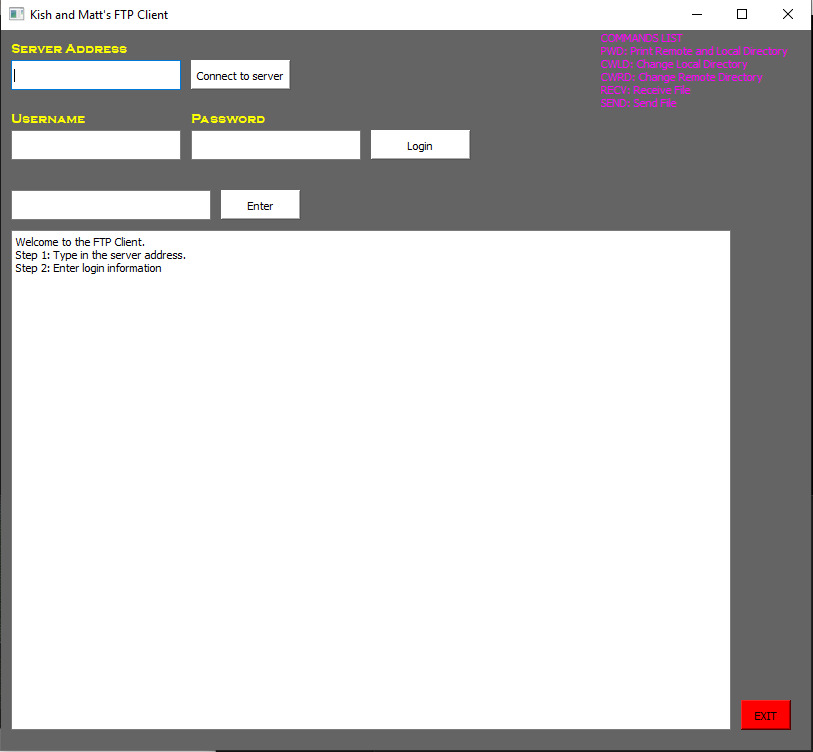
\includegraphics[scale=0.8]{GUI.png}
\caption{Designed GUI in \code{PyQt5}}
\label{fig: GUI}
\end{figure}


\pagebreak
\section{Implemented Commands and Reply Codes}
\label{app: Commands}


\begin{table}[h!]
\caption{Table detailing the implemented commands and reply codes}
\label{tab}
\begin{tabular}{|l|l|l|}
\hline
\multicolumn{1}{|c|}{{\ul \textbf{Command}}} & \multicolumn{1}{c|}{{\ul \textbf{Description}}} & \multicolumn{1}{c|}{{\ul \textbf{Reply Code}}} \\ \hline
USER & User identification needed by server before providing access to file system & \begin{tabular}[c]{@{}l@{}}501 Syntax error in parameters or arguments.\\ 331 User name okay, need password.\end{tabular} \\ \hline
PASS & Authenticates user password & \begin{tabular}[c]{@{}l@{}}501 Syntax error in parameters or arguments.\\ 503 Bad sequence of commands. \\ 230 User logged in, proceed.\end{tabular} \\ \hline
CWD & Changes working directory to new directory specified user & \begin{tabular}[c]{@{}l@{}}550 Requested action not taken. File unavailable\\ 250 Requested file action okay, completed.\end{tabular} \\ \hline
CDUP & Changes the working directory to home directory. & 200 Command okay. \\ \hline
QUIT & Terminates a user connection & 221 Service closing control connection. Goodbye \\ \hline
PORT & Specifies the data port to be used during data transmission & 200 Command okay. Get Port \\ \hline
PASV & Requests the FTP server listen on the specified data port & 227 Entering Passive Mode \\ \hline
TYPE & Specifies the file type to be retrieved or stored & \begin{tabular}[c]{@{}l@{}}200 Command okay.\\ 501 Syntax error in parameters or arguments.\end{tabular} \\ \hline
STRU & Specifies the file structure to be retrieved or stored & \begin{tabular}[c]{@{}l@{}}200 Command okay.\\ 502 Command not implemented.\end{tabular} \\ \hline
MODE & Specifies data transfer modes for transmission & \begin{tabular}[c]{@{}l@{}}200 Command okay. \\ 502 Command not implemented.\\ 501 Syntax error in parameters or arguments.\end{tabular} \\ \hline
LIST & \begin{tabular}[c]{@{}l@{}}Returns a list of the contents of a specified directory.\\ The list contains the type of files included in the directory.\end{tabular} & \begin{tabular}[c]{@{}l@{}}530 User not logged in.\\ 550 Requested action not taken. File unavailable\\ 150 File status okay; about to open data connection.\\ 226 Closing data connection. Requested file action successful\end{tabular} \\ \hline
PWD & Returns the current working directory & 257 PATHNAME created \\ \hline
RETR & Enables the download capabilities of the specified file name & \begin{tabular}[c]{@{}l@{}}150 File status okay; about to open data connection.\\ 226 Transfer complete.\end{tabular} \\ \hline
STOR & Enables the upload capabilities of the specified file name & \begin{tabular}[c]{@{}l@{}}530 Not logged in.\\ 150 File status okay; about to open data connection.\\ 226 Transfer completed.\end{tabular} \\ \hline
NOOP & Gives the client ping capabilities when attempting to access the server & 200 Command okay \\ \hline
\end{tabular}
\end{table}

\pagebreak
\section{Results}
\label{app: Results}

\begin{figure}[h!]
\renewcommand{\thefigure}{\arabic{figure}}
\centering
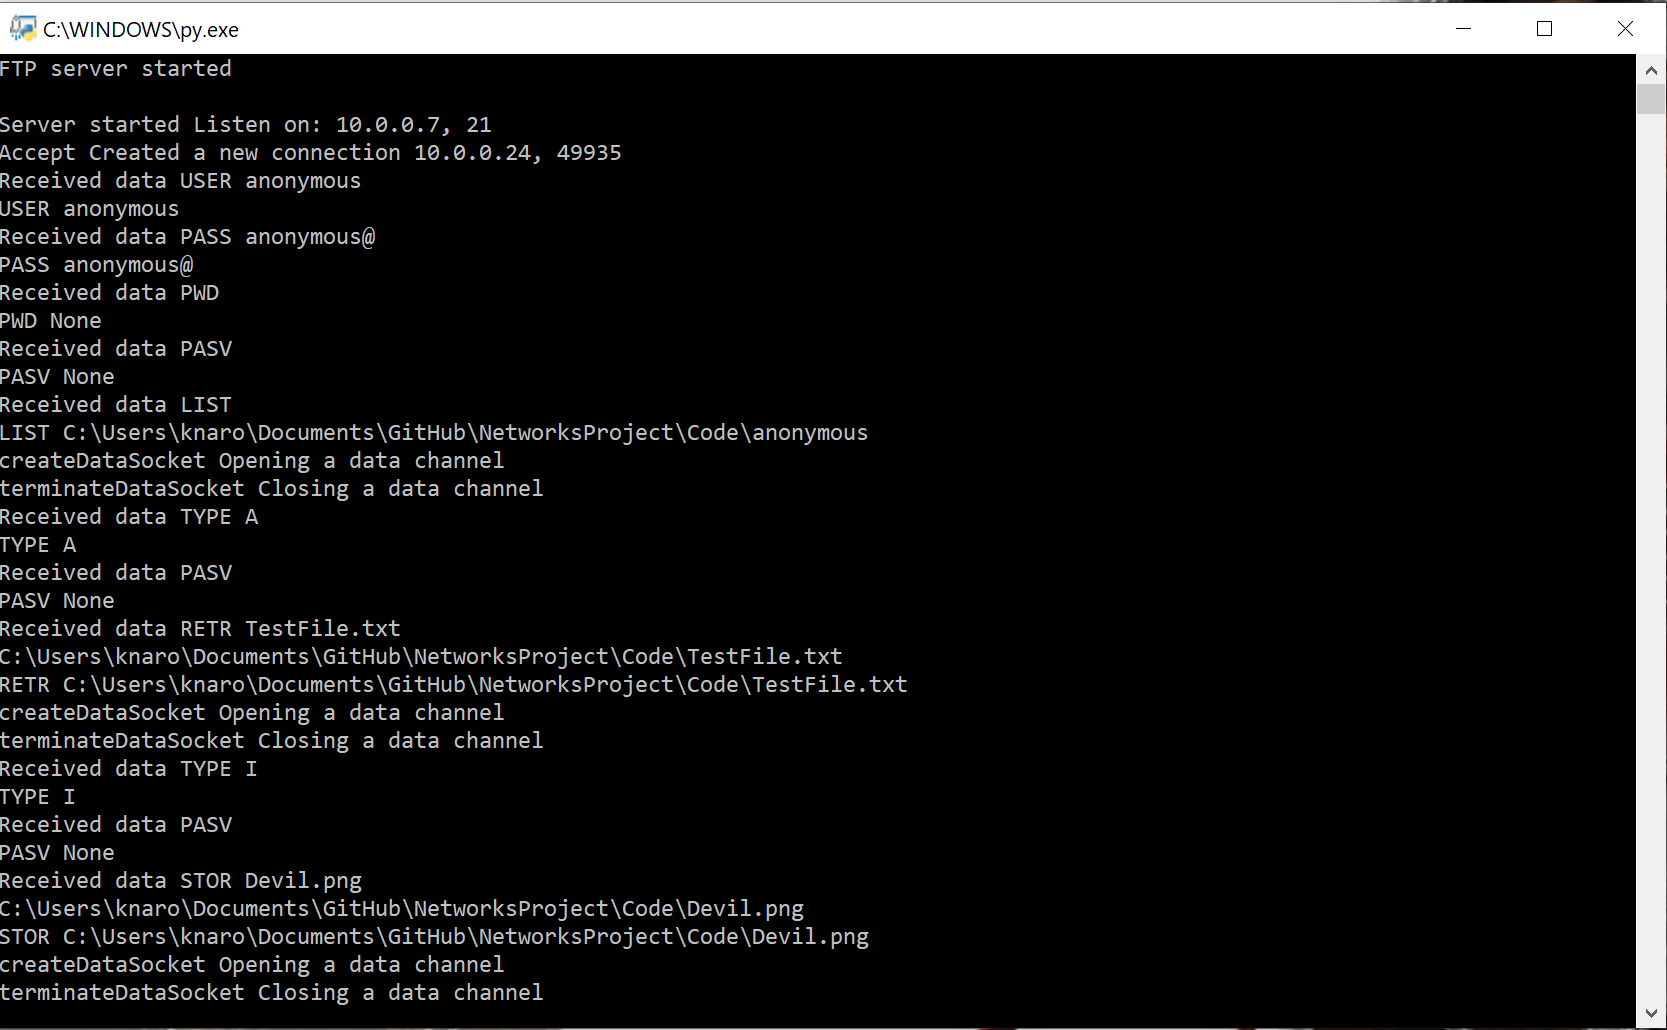
\includegraphics[scale=0.6]{Server.png}
\caption{Server log on host \code{10.0.0.7}}
\label{fig: Server log}
\end{figure}

\begin{figure}[h!]
\renewcommand{\thefigure}{\arabic{figure}}
\centering
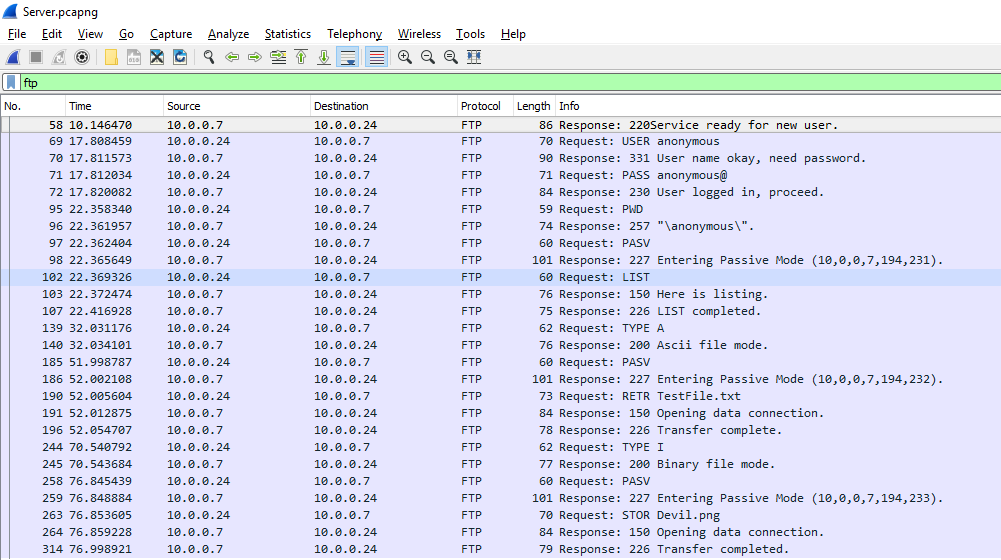
\includegraphics[scale=0.6]{ServerWireshark.png}
\caption{Wireshark trace of implemented client (\code{10.0.0.24}) and implemented server (\code{10.0.0.24})}
\label{fig: Server Wireshark}
\end{figure}

\begin{figure}[h!]
\renewcommand{\thefigure}{\arabic{figure}}
\centering
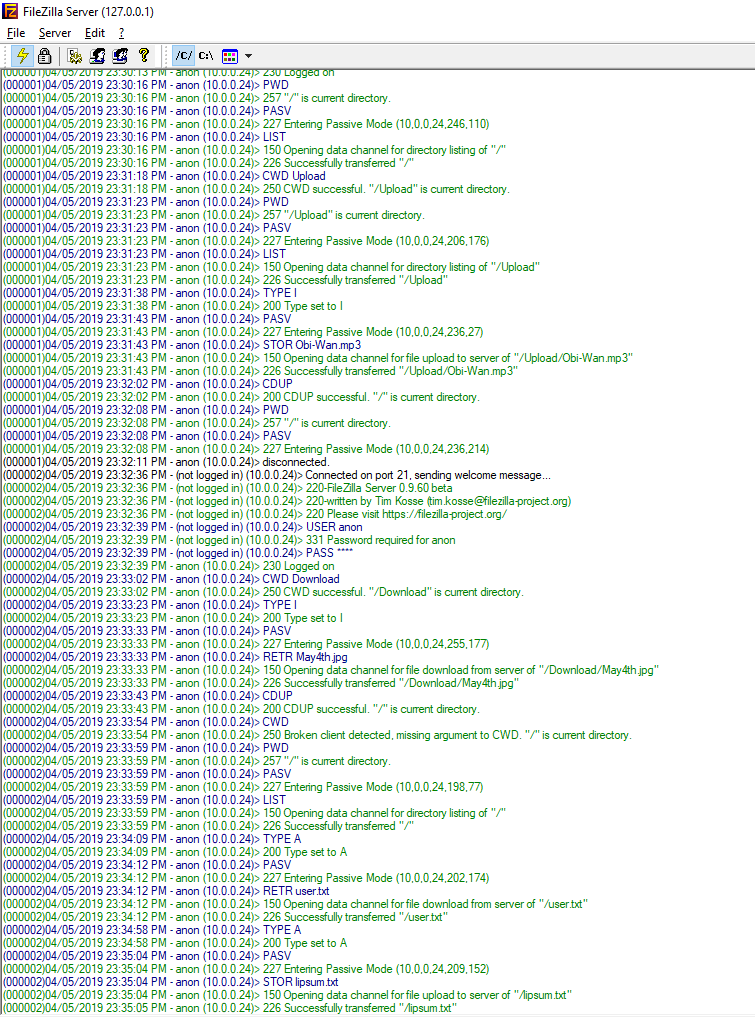
\includegraphics[scale=0.9]{FileZilla.png}
\caption{FileZilla log}
\label{fig: FileZilla log}
\end{figure}

\begin{figure}[h!]
\renewcommand{\thefigure}{\arabic{figure}}
\centering
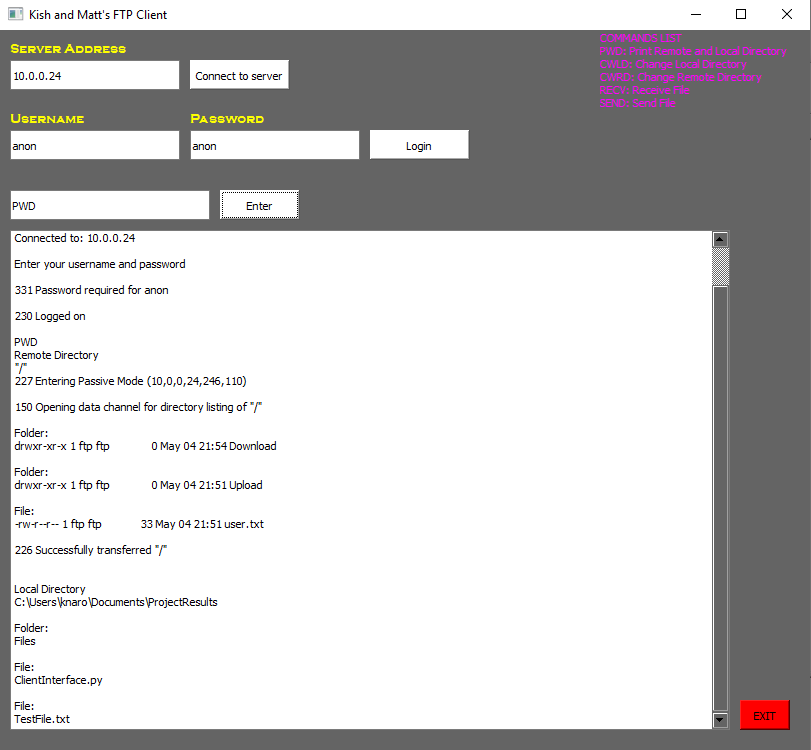
\includegraphics[scale=0.8]{FileZillaGUI.png}
\caption{GUI output of printing the current directories}
\label{fig: FileZilla GUI}
\end{figure}

\begin{figure}[h!]
\renewcommand{\thefigure}{\arabic{figure}}
\centering
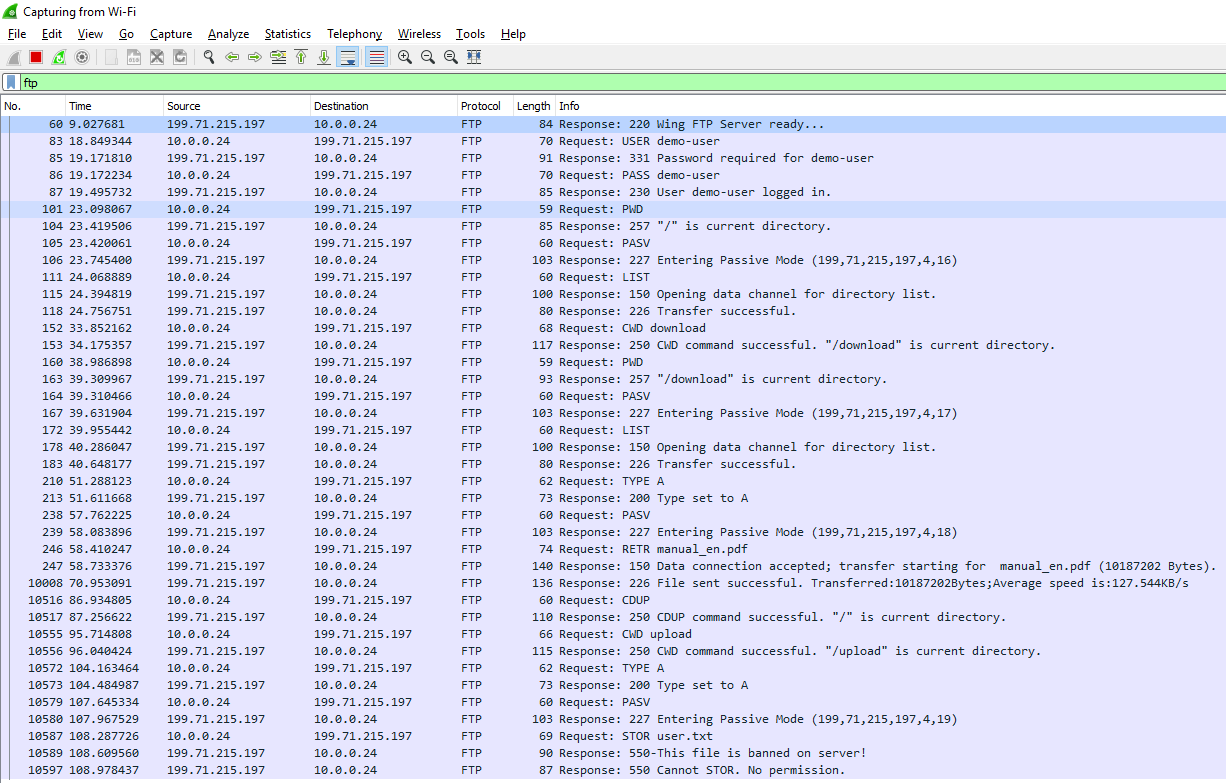
\includegraphics[scale=0.55]{WftpWireshark.png}
\caption{FileZilla log}
\label{fig: Wftp Wireshark}
\end{figure}

\begin{figure}[h!]
\renewcommand{\thefigure}{\arabic{figure}}
\centering
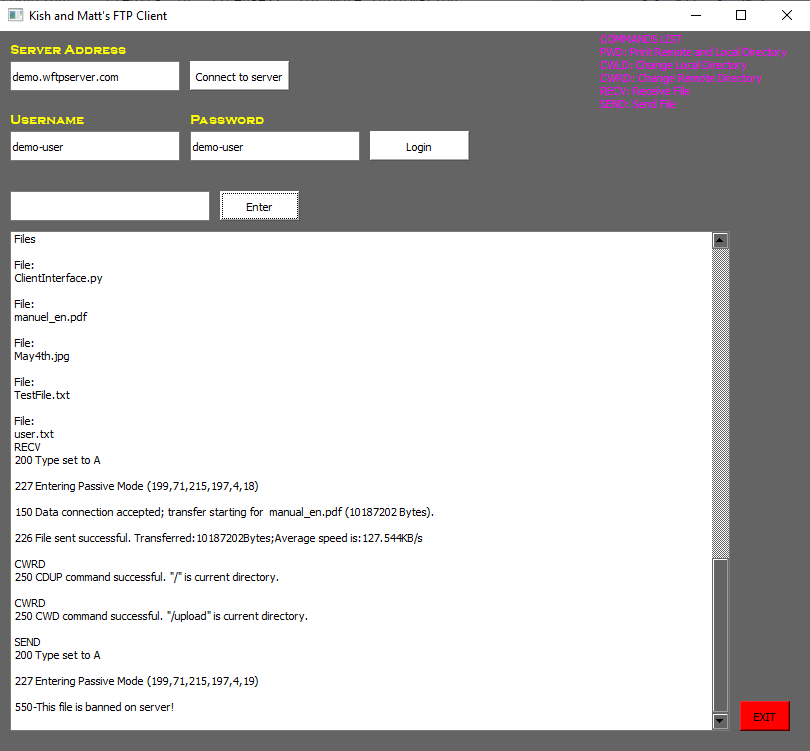
\includegraphics[scale=0.8]{WftpGUI.png}
\caption{GUI output after downloading a file from the server (\code{demo.wftpserver.com})}
\label{fig: Wftp GUI}
\end{figure}

\end{appendices}
% that's all folks
\end{document}


